\documentclass{article}
\usepackage{amsthm, amssymb, latexsym, amsmath, amsbsy, graphicx, epsfig}
\usepackage{ mathrsfs }
\usepackage{ textcomp }
\usepackage{titling}
\usepackage[top=1in, left=2in, right=2in]{geometry}
\usepackage{caption}
\graphicspath{{figures/}}


\renewcommand{\baselinestretch}{2} 
\setlength{\parskip}{1em} 
\setlength{\parindent}{0pt} 
\title{\textbf{Brain Teaser of the Week - The Aldens Handshake Problem}}
\author{Robert T Kohn}
\date{April 11th  2025}
\begin{document}
\maketitle

\begin{center}
\vspace{-3.033em}
\noindent\rule{0.7\linewidth}{0.5pt}

\textbf{\large The Question}
\end{center}
\begin{quotation}
Mr.\ and Mrs.\ Alden hosted a party for at least one other couple.  Later
Mr.\ Alden asked everyone else (including his wife) how many hands each had shaken. He found that
no two people gave him the same answer. If no one shook their own hand, no partners shook hands, and no two
people shook hands more than once, how many hands did Mrs.\ Alden shake?
\end{quotation}


\begin{center}
\textbf{\large The Requirements}
\end{center}
\begin{itemize}
    \item \textbf{Each person who Mr.\ Alden asked has a unique hand shake count.} 
\item \textbf{There is at least one other couple there.} 
    \item \textbf{No self or partner handshakes.} 
\item \textbf{No two people shook hands more than once.} 
\end{itemize}

\begin{center}
\textbf{\large The Answer?}

Shockingly, the answer is that Mrs.\ Alden shook the same amount of hands as the amount of couples at the party.
\end{center}

\begin{center}
\textbf{\large Proving this Claim}
\end{center}
\vspace{-3.033em}
\subsection*{Real World Comparison to Guide Intuition}
It's best to start small to see the bigger pattern. 
Imagine that the Aldens host only one other couple. Then there are 4 people at the party but because Mr.\ Alden is uninterested with how many hands he shook, there are only 3 people whose handshake count matters. Since we know that everyone Mr.\ Alden asked has a unique handshake count, there are  only 3 possible handshake combinations. The 3 people Mr.\ Alden asked must have given the answer that they shook no hands, 1 hand, or 2 hands. The other couple at the party must have one partner who shook everyone but their partner's hand. Let's refer to them as the social butterfly. While the other partner must have shook 0 hands and can be called a ghost. Hence, Mrs.\ Alden has to be the last part of the combination and has to have shook one hand because she cannot shake her husband's hand.
Now, let's apply this concept to 2 other couples. This means there are only 5 people whose handshake matters. As we know, each person Mr.\ Alden asked has a unique hand shake count so they could have only shook 0 hands, 1 hand, 2 hands, 3 hands, or 4 hands. Let's imagine the new couple consists of a bigger social butterfly and an even shyer ghost. They would account for 0 and 4 handshakes. Which means the other couple must have shook 3 hands and 1 hand. As a result, Mrs.\ Alden again shakes two hands to fill the gap. In both cases, Mrs. Alden shook the same number of hands as couples at the party. And, this pattern isn’t a coincidence, it scales perfectly.

\begin{figure}[htbp]
    \centering
    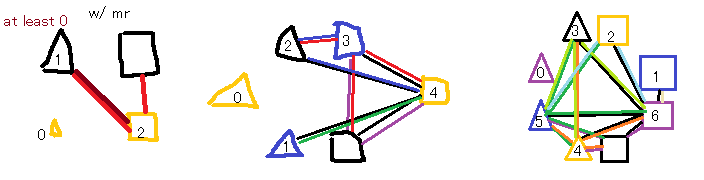
\includegraphics[width=0.85\textwidth]{alden_handshake_model.png}
    \caption*{Graphical model of handshake distribution for $n \le 2$ couples}
\end{figure}

\subsection*{Using the Principle Mathematical Induction to Confirm Mrs.\ Alden Shook the Same Number of Hands as the Amount of Couples}
Now to generalize the logic using the Principle of Mathematical Induction. The Principle of Mathematical Induction proves a statement for all natural numbers. The first step is by verifying that when the basic conditions are met that the outcome is what is expected. We just proved this above so let's work on generalizing.
Suppose for some arbitrary and unknown amount of other couples and lets call it \textbf{k}, Mrs.\ Alden shakes  \textbf{k} hands.
To see why this holds for any number of couples, let’s consider a domino effect. For the sake of this argument, let's imagine there is an additional couple, with the biggest social butterfly and shyest ghost, added to the \textbf{k} couples. So, there are now \textbf{2k} and 3 people whose handshakes matter. But, there is one less possible handshake because of the ghost. So, Mrs.\ Alden has to have shook \textbf{k} hands like before and also the social butterfly's hand to combine for \textbf{k+1} hands shook, this is the same amount couples at the party.
Therefore, using the Principle of Mathematical Induction, we can conclude that Mrs. Alden shakes the same number of hands as there are couples at the party.

\end{document}
